\chapter{REFERENCIAL TEÓRICO}
Para o entendimento e progresso deste trabalho, faz-se necessária a compreensão de conceitos relacionados a Séries Temporais, incluindo suas Técnicas e Modelagem, Análise de Dados Meteorológicos, Fontes de Dados Meteorológicos, Aplicações de Séries Temporais em Meteorologia, Ferramentas e Métodos Estatísticos, bem como a Análise Exploratória de Dados, Redes Neurais e Séries Temporais com Redes Neurais. 

\section{SÉRIES TEMPORAIS}
    Muitas pessoas, em algum momento, já imaginaram como seria prever o futuro e ter acesso a informações sobre eventos 
    ou situações de suas vidas. Essa curiosidade reflete um desejo universal, mas também uma necessidade presente em 
    diversas áreas, como na gestão governamental, no setor financeiro e em contextos sociais. Nesse cenário, surge o 
    conceito de Série Temporal, definido como um conjunto de observações organizadas sequencialmente no tempo, 
    representadas por \( x_t \), com cada valor correspondente a um instante específico \(t\) \cite{box2015}. O estudo de 
    Séries Temporais permite não apenas compreender as características de fenômenos que evoluem ao longo do tempo, mas 
    também desenvolver e ajustar modelos estatísticos capazes de explicar ou prever o comportamento dos dados 
    observados.
    
    De acordo com CITAR O LIVRO Introduction to Time Series and Forecasting, séries temporais podem ser classificadas 
    discretas e continuas, uma série temporal é discreta quando o conjunto \( t_0 \) de tempos em que as observações 
    são feitas é um conjunto discreto, como o caso de observações que são realizadas em um determinado intervalo de 
    tempo fixo. Sendo denotada por:
    \begin{equation}
        \{X_t : t \in T\}, \quad T = \{t_1, \dots, t_n\}
    \end{equation}
    
    
    
    E seríes temporais continuas quando suas observações são obtidas continualmente 
    no tempo. 
    \begin{equation}
        \{X(t) : t \in T\}, \quad T = \{t : t_1 < t < t_2\}
    \end{equation}
        

    
    Ao iniciar a análise de uma série temporal é de alta valia utilizar de gráficos criados sequencialmente no tempo,
    visto que isso pode revelar determinados padrões de comportamento e algumas características que podem estar 
    presentes nos dados, como tendência, sazonalidade, ciclidade e ruído também chamado de erro aleatório (Citar ufrb). 

    \subsection{DECOMPOSIÇÃO CLÁSSICA}

        A tendência ($\mu_t$) é falar o que é a tendência \\
        
        A ciclidade ($\psi_t$) pode ser \\
        
        A sazonalidade ($\gamma_t$) pode ser \\
        
        O ruído ($\epsilon_t$) é 

        %mostrar fórmula



\section{REDES NEURAIS}
%Falar brevemente
    O cérebro humano é um computador de grande complexidade, não linear e paralelo, 
    composto por cerca de 10 bilhões de neurônios, cada um conectado com outros 10 
    bilhões de neurônios. Em sua composição existe o corpo da célula também chamado de 
    soma, e canais da saída e entrada (dendritos e axônios) que conectam os neurônios, 
    dendritos também são chamadas zonas receptivas e axônios de linhas de transmissão. 
    Cada neurônico recebe informações eletroquimicas de outros neurônios nos dendritos 
    através dos axônios. Se as somas dessas entradas elétricas for suficientemente forte 
    para ativar o neurônio, um sinal eletroquímico ao longo do axônio, possuindo a 
    habilidade de organizar os neurônios, um dos seus componentes integradores, para 
    assim realizar várias formas de processamento de forma mais rápida que os 
    computadores digitivas convencionais. (CITAR O O LIVRO).

    A Figura \ref{fig:celula_piramidial} mostra a estrutura do neurônio:
    \begin{figure}[!htb]
        \centering
        \caption{Célula piramidial.}
        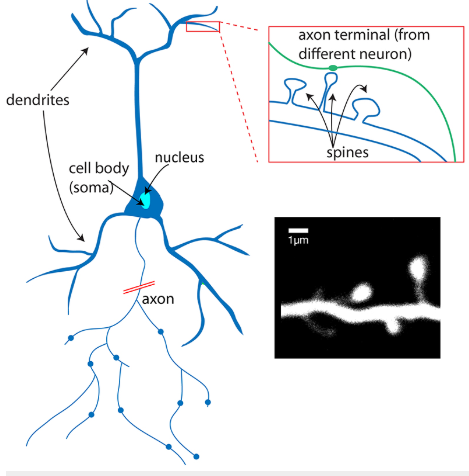
\includegraphics[scale=0.5]{celula-piramidial.png}\\
        {\footnotesize Fonte: The University Of Queensland.}\
        \label{fig:celula_piramidial}
    \end{figure}
        
    \subsection{HISTÓRICO}
        % No livro de Fausett L.-Fundamentals of Neural Networks_ Architectures, Algorithms, and Applications (1994).pdf 
        As redes neurais são frequentemente consideradas um complemento à computação tradicional. Curiosamente, 
        John von Neumann, amplamente reconhecido como o pai da computação moderna devido à sua proposta da arquitetura 
        que possibilitou a criação do computador de programa armazenado, demonstrava grande interesse em modelar o 
        funcionamento do cérebro humano. Esse interesse levantou debates entre pesquisadores sobre a possível interação 
        entre as ideias de von Neumann e os primórdios das redes neurais. Alguns estudiosos destacam indícios que 
        sugerem a visão de von Neumann sobre as direções futuras do desenvolvimento dos computadores (CITAR O LIVRO).

        \subsubsection{PERCEPTRONS}
            Em 1958, um psicólogo chamado Rosenblatt, publicou um artigo que descrevia pela primeira vez de forma a
            algoritmica o funcionamento de uma rede neural. Dessa forma, inspirando diversos pesquisadores a dedicarem
            seus esforços de pesquisas envolvendo a temática de redes neurais e seus diferentes aspescos na década de 
            1960 à 1970 (CITAR LIVRO Neural Networks and Learning Machines, Third Edition). 
            

        \subsubsection{ADELAIDE}

        \subsubsection{BACKPROPAGATION}
      
        
    \subsection{COMPONENTES DAS REDES NEURAIS}
        %

    \subsection{APRENDIZADO EM REDES NEURAIS}
    \subsection{ARQUITETURAS}
    %Falar o que é e botar uma imagem em todas
        \subsubsection{FEED-FORWARD}
        \subsubsection{MULTI LAYER PERCEPTRON}
        \subsubsection{REDES NEURAIS RECORRENTES}
        \subsubsection{REDES NEURAIS CONVOLUCIONAIS}
        \subsubsection{LONG SHORT-TERM MEMORY (LSTM)}
    

%Talvez por na metodologia
\section{DADOS METEOROLÓGIOCOS}

    Para a aplicação de modelos de previsão, é essencial dispor de uma quantidade significativa de dados para o 
    treinamento, validação e teste do modelo, bem como para a inferência dessas informações sobre a população como um 
    todo. No Brasil, o Instituto Nacional de Meteorologia (INMET) é o órgão responsável pelo Banco de Dados 
    Meteorológicos (BDMEP), planejado para coletar, armazenar, processar e disponibilizar dados e informações sobre 
    variáveis meteorológicas. 
    
    Esses dados podem ser gerados localmente, por meio de estações meteorológicas convencionais ou automáticas, 
    ou captados remotamente, utilizando sensores orbitais, radares, entre outros dispositivos (VIANNA et al., 2017). 
    O Banco de Dados Meteorológicos para Ensino e Pesquisa (BDMEP), em particular, reúne informações meteorológicas 
    diárias provenientes das estações da rede do INMET, seguindo as normas técnicas da Organização Meteorológica 
    Mundial (INMET, s.d.).